\documentclass{article}
\usepackage{amsfonts, amsbsy, amssymb, amsmath, graphicx, float, subfigure}

\tolerance=5000 
\textwidth=16.6 cm 
\oddsidemargin=-.04 cm
\evensidemargin=-.04 cm 
\topmargin=-1.3 cm 
\textheight=22.9 cm




\newtheorem{definition}{Definition}
\newtheorem{assumption}{Assumption}
\newtheorem{hyp}{Hypothesis}
\newtheorem{theorem}{Theorem}
\newtheorem{lemma}{Lemma}[section]
\newtheorem{corollary}{Corollary}[section]
\newtheorem{proposition}{Proposition}[section]



\begin{document}







\section*{A Two Degree-of-Freedom Index One Saddle--A  Saddle-Center Equilibrium Point}
\


We consider  a quadratic 2 DoF  Hamiltonian:


\begin{equation}
H = \underbrace{\frac{\lambda}{2} \left(p_1^2 - q_1^2 \right)}_{H_1} + \underbrace{\frac{\omega}{2} \left(p_2^2 + q_2^2 \right)}_{H_2}, \quad \lambda, \, \omega >0,
\label{ham2}
\end{equation}

\noindent
with the corresponding Hamilton's equations given by:

\begin{eqnarray}
\dot{q}_1 & = & \frac{\partial H}{\partial p_1}= \lambda p_1, \nonumber \\
\dot{p}_1 & = & -\frac{\partial H}{\partial q_1}= \lambda q_1, \nonumber \\
\dot{q}_2 & = & \frac{\partial H}{\partial p_2}= \omega p_2, \nonumber \\
\dot{p}_2 & = & -\frac{\partial H}{\partial q_2}= -\omega q_2, 
\label{hameq2}
\end{eqnarray}

\noindent
These equations have an equilibrium point of saddle-center equilibrium type (index one saddle) at the origin.
In Fig. \ref{fig:2 dof saddle} a) we show contours  of the potential energy and in Fig. \ref{fig:2 dof saddle} b) we show the phase portrait corresponding to \eqref{ham2}. 
Since the Hamiltonians $H_1$ and $H_2$ are uncoupled we can sketch the phase portraits for each separately.  and discuss the distribution of total energy between each DoF in a simple manner.



\begin{figure}[htb!]
\begin{center}
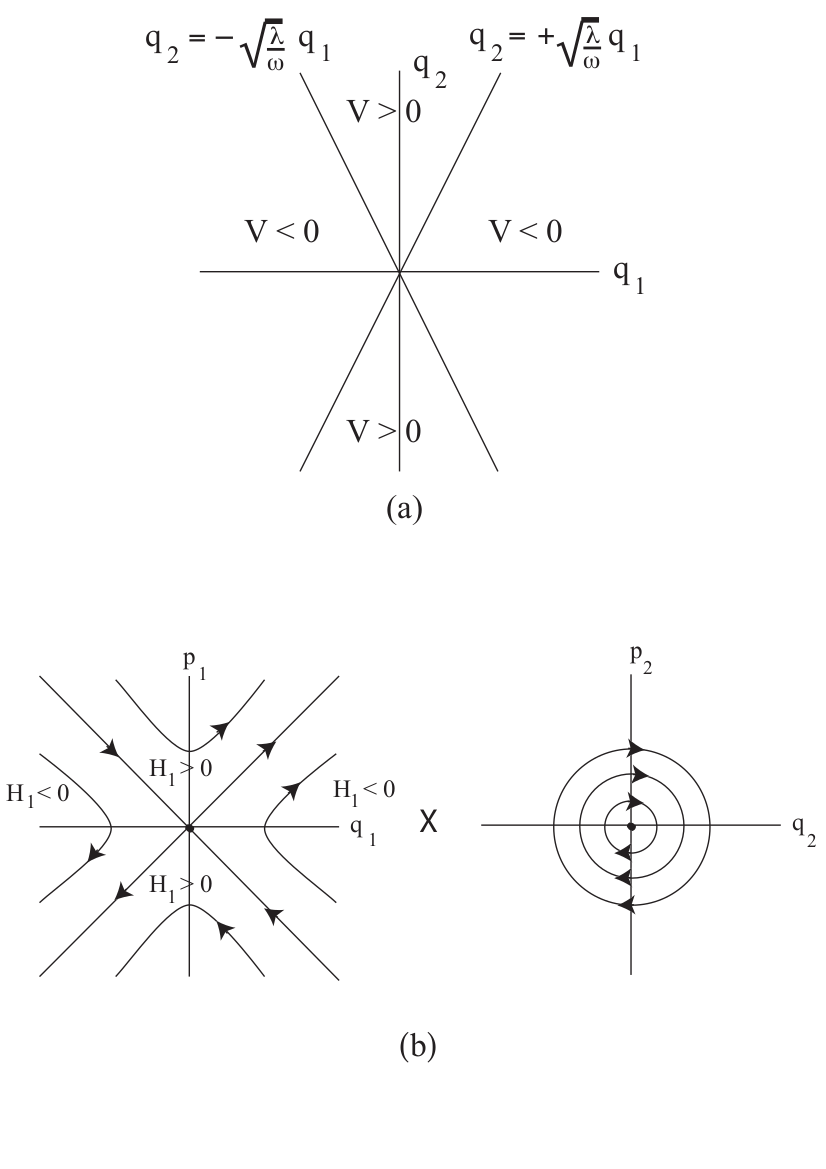
\includegraphics[width=6.0cm]{fig_2_dof_saddle.png}
\end{center}
\caption{a) Contours of the potential energy, $V(q_1, q_2) =-\frac{\lambda}{2} q_1^2 + \frac{\omega}{2} q_2^2$,  denoting the sign of $V(q_1, q_2) = \mbox{constant}$. b) The phase space for the two DoF saddle defined by \eqref{hameq2}.}
\label{fig:2 dof saddle}
\end{figure}



Note that trajectories corresponding to $H_1$ can become unbounded and trajectories corresponding to $H_2$ are bounded.  Hence in  this system reaction occurs when  the $q_1$ coordinate of a trajectory changes sign. Therefore, a `'natural'' dividing surface would be $q_1 =0$. This is a three dimensional surface in the four dimensional phase space. We want to examine it's structure more closely and, in particular, its' intersection with a fixed energy surface. We will also utilize terminology from chemistry by referring to  $H_1$ as the `'reactive mode'' and $H_2$ is the `'bath mode''


First, note that for reaction to occur we must have $H_1 >0$, since the $q_1$ component of reacting trajectories changes sign. Also, it is clear  from  the form of $H_2$ that $H_2 \ge 0$. Therefore, for reaction we must have $H = H_1 + H_2 >0$. The energy surface is given by:

\begin{equation}
\frac{\lambda}{2} \left(p_1^2 - q_1^2 \right) + \frac{\omega}{2} \left(p_2^2 + q_2^2 \right) = H_1 + H_2 = H > 0, \quad H_1 > 0, \, H_2 \ge 0.
\label{2DoFES}
\end{equation}

\noindent
The intersection of $q_1=0$ with this energy surface is given by:



\begin{equation}
\frac{\lambda}{2} \, p_1^2  + \frac{\omega}{2} \left(p_2^2 + q_2^2, \right) = H_1 + H_2 = H > 0, \quad H_1 > 0, \, H_2 \ge 0.
\label{2DoDS}
\end{equation}

\noindent
This is the isoenergetic DS. It has the form of a 2-sphere in the four dimensional $(q_1, p_1, q_2, p_2)$ space. It has two `'halves'' corresponding to the forward and backward reactions, respectively:

\begin{equation}
p_1 = + \sqrt{\frac{2}{\lambda}} \sqrt{H_1 + H_2 - \frac{\omega}{2} \left(p_2^2 + q_2^2 \right) }, \quad \mbox{forward DS},
\end{equation}

\begin{equation}
p_1 = - \sqrt{\frac{2}{\lambda}} \sqrt{H_1 + H_2 - \frac{\omega}{2} \left(p_2^2 + q_2^2 \right) }, \quad \mbox{backward DS}.
\end{equation}

\noindent
Since $\dot{q}_1 = \lambda p_1$ it is clear that the DS, being defined by $q_1=0$ is a surface  having the `'no-recrossing'' property.


The forward and backward DS `'meet'' at  $p_1 =0$:

\begin{equation}
 \frac{\omega}{2} \left(p_2^2 + q_2^2, \right) = H_1 + H_2 \ge  0,   \mbox{NHIM},
\end{equation}

\noindent
which is an unstable periodic orbit in the $p_2-q_2$ plane. This is   the NHIM for this 2 DoF system. In this particular example, and in the case where the NHIM is one orbit, normal hyperbolicity is easy to understand. The orbit is normally hyperbolic if it is of saddle-type stability. From \eqref{hameq2}, we see that the coordinates `'normal'' to the periodic orbit are $q_1=p_1$, and the dynamics in these coordinates is linear and of saddle type.









\end{document}


